The Compact C Type Format (CTF) encapsulates all of the information
needed by OpenDTrace to understand C language types such as integers,
strings, floats and structures.  The goal of having another section
just for C type information is to provide a compact representation of
the information that usually appears in the debugging sections of
object files and executables.  CTF only contains data types it
does not contain other debugging infromation, which allows it to be
far more compact.  The debugging sections on a debug build of FreeBSD
in 2017 take up 78 megabytes of space, while the CTF section in the
same kernel take up only 800 kilobytes. 

\section{On Disk Format}
\label{sec:ctf-on-disk-format}

CTF data is stored in its own ELF section within an object file or
executable.  It is meant to be stored in a format that is both compact
and which is properly aligned so that it can be accessed using the
\texttt{mmap} (2) system call.

\begin{figure}[h]
  \centering
  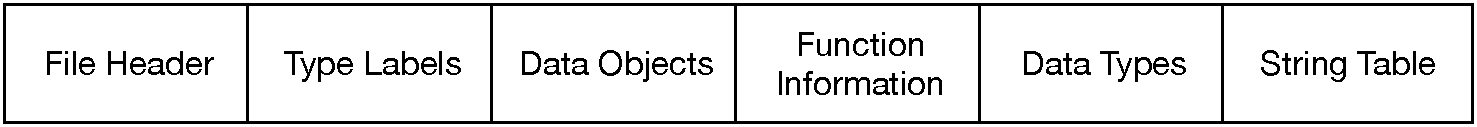
\includegraphics[width=.8\textwidth]{ctf-stable-format}
  \caption{CTF Stable Storage Format}
  \label{fig:ctf-stable-storage-format}
\end{figure}

Figure~\ref{fig:ctf-stable-storage-format} shows all of the components
of the CTF section as they would be found on stable storage.  The file
header stores a magic number and version information, encoding flags,
and the byte offset of each of the sections relative to the end of the
header itself.  As of this writing the most current version of CTF is
version two (2).  The preamble, including the magic number, version
and flags, take up the first 32 bits of the header, the remaining
fields take up 32 bits each, independent of the word size of the
architecture.

\begin{figure}
  \centering
  \begin{bytefield}[endianness=big,bitformatting=\scriptsize]{32}
    \bitheader{0,8,16,31} \\
    \bitbox{16}{magic}
    \bitbox{8}{version}
    \bitbox{8}{flags}\\
    \bitbox{32}{reference to parent label}\\
    \bitbox{32}{reference to basename of parent}\\
    \bitbox{32}{label section offset}\\
    \bitbox{32}{function section offset}\\
    \bitbox{32}{type section offset}\\
    \bitbox{32}{string section offset}\\
    \bitbox{32}{size of string section (bytes)}\\
  \end{bytefield}
  \caption{Overall CTF section encoding}
  \label{fig:ctf-overall}
\end{figure}

The CTF section makes heavy use of references between the sub-sections
to fully describe the datatypes in a program as well as the functions,
the function's argument list, and the function's return value.  The
\verb|data objects| and \verb|functions| sections depend upon the
\verb|type| section, which encodes all of the datatypes that have
been during the CTF conversion process.  Each type has a unique number
and name, as well as a size and encoding.  Types may refer to other,
more primitive types by use of a reference, e.g. a \verb|uint32_t|
will actually refer to a \verb|unsigned int|.  Types are broken up by
what they represent, referred to as their \emph{kind}.

\begin{table}
  \centering
  \begin{tabular}{|l|l|}
    \hline
    \verb|CTF_K_UNKNOWN|    & unknown type (used for padding) \\
    \verb|CTF_K_INTEGER|    & variant data is \verb|CTF_INT_DATA()| (see below)\\
    \verb|CTF_K_FLOAT|      & variant data is \verb|CTF_FP_DATA()| (see below)\\
    \verb|CTF_K_POINTER|    & \verb|ctf_type| is referenced type\\
    \verb|CTF_K_ARRAY|      & variant data is single \verb|ctf_array_t|\\
    \verb|CTF_K_FUNCTION| & \verb|ctt_type| is return type\\
                            &  variant data is list of argument types\\
                            & (\verb|ushort_t|'s)\\
    \verb|CTF_K_STRUCT|     & variant data is list of \verb|ctf_member_t|'s\\
    \verb|CTF_K_UNION|      & variant data is list of \verb|ctf_member_t|'s\\
    \verb|CTF_K_ENUM|       & variant data is list of \verb|ctf_enum_t|'s\\
    \verb|CTF_K_FORWARD|    & no additional data; \verb|ctt_name| is tag\\
    \verb|CTF_K_TYPEDEF|    & \verb|ctf_type| is referenced type\\
    \verb|CTF_K_VOLATILE|   & \verb|ctf_type| is base type\\
    \verb|CTF_K_CONST|      & \verb|ctf_type| is base type\\
    \verb|CTF_K_RESTRICT|   & \verb|ctf_type| is base type\\
    \hline
  \end{tabular}
  \caption{Kinds of CTF Base Types}
  \label{tbl:ctf-kinds}
\end{table}

Table~\ref{tbl:ctf-kinds} lists the kinds of base data types that are
encoded by CTF.  Complex data types, such as structures, are also
contained in the \verb|types| section, and are encoded as a structure
with a name that references the string table.

\begin{figure}
  \centering
  \begin{bytefield}[endianness=big,bitformatting=\scriptsize]{32}
    \bitheader{0,16,31} \\
    \bitbox{32}{name}\\
    \bitbox{16}{info}
    \bitbox{16}{size or type}\\
  \end{bytefield}
  \caption{A simple type}
  \label{fig:ctf-stype}
\end{figure}

A simple type, one who's size is less than 64 Kbytes, is stored in a
\verb|ctf_stype|, shown in Figure~\ref{fig:ctf-stype}.  The
\verb|name| is a reference to a string in the string table.  The
\verb|info| field is encoded differently for each type, as will be
explained fully in the rest of this chapter.  The last field is either
the size, in bytes, of the structure or it is a reference to another
type, encoded using the referenced type's ID.  The majority of types
in a C program will fit within a \verb|ctf_stype|.

\begin{figure}
  \centering
  \begin{bytefield}[endianness=big,bitformatting=\scriptsize]{32}
    \bitheader{0,16,31} \\
    \bitbox{32}{name}\\
    \bitbox{16}{info}
    \bitbox{16}{size or type}\\
    \bitbox{32}{high 32 bits of size (in bytes)}\\
    \bitbox{32}{low 32 bits of size (in bytes)}\\
  \end{bytefield}
  \caption{A large type}
  \label{fig:ctf-type}
\end{figure}

Types that are larger than 64Kbytes are encoded using a
\verb|ctf_type| structure, shown in Figure~\ref{fig:ctf-type}.  The
\verb|name| and \verb|info| fields of this, larger, \verb|ctf_type|
are the same as the smaller \verb|ctf_stype|, but the \verb|size|
field is always set to \verb|CTF_LSIZE_SENT|, the sentinal value that
tells the consumer that this is a larger structure.  A \verb|ctf_type|
structure can encode an extremely large type, since it provides 64
bits for the size, and that size is expressed in bytes.

\begin{figure}
  \centering
  \begin{bytefield}[endianness=big,bitformatting=\scriptsize]{16}
    \bitheader{0,9,10,15}\\
    \bitbox{5}{kind}
    \bitbox{1}{r}
    \bitbox{10}{vlen}
  \end{bytefield}
  \caption{Info field encoding}
  \label{fig:ctf-info-field}  
\end{figure}

The \verb|info| field, shown in Figure~\ref{fig:ctf-info-field}, is
further broken down into a number of sub-fields which encoded the
\verb|kind|, \verb|vlen| (variable length) and whether or not this is
a root type \verb|isroot|.

Each of the integral types, such as integers, floats, pointers, arrays, etc.
has its own encoding.  Integers are the simplest type and are unsigned by
default.  An integer type is encoded in a single, 32 bit, field, as
seen in Figure~\ref{fig:ctf-integral}.

\begin{figure}
  \centering
  \begin{bytefield}[endianness=big,bitformatting=\scriptsize]{32}
    \bitheader{0,16,24,31} \\
    \bitbox{8}{flags}
    \bitbox{8}{offset}
    \bitbox{16}{size in bits}
  \end{bytefield}
  \caption{Integral type encoding}
  \label{fig:ctf-integral}
\end{figure}

The \verb|flags| field indicates whether the integer is signed,
contains character data, is a boolean or is to be displayed
with a vargs style of formatting.

Floating point numbers have the exact same fields to describe them
but a larger number of possible flags, to match the larger
number of ways in which floating point numbers may be stored.
The flags and descriptions of the currently supported floating
point encodings are given in Table~\ref{tbl:ctf-kinds}.

\begin{table}
  \centering
  \begin{tabular}{|l|l|}
    \hline
    \verb|CTF_FP_SINGLE|   & IEEE 32-bit float encoding\\
    \verb|CTF_FP_DOUBLE|   & IEEE 64-bit float encoding\\
    \verb|CTF_FP_CPLX|     & Complex encoding\\
    \verb|CTF_FP_DCPLX|    & Double complex encoding\\
    \verb|CTF_FP_LDCPLX|   & Long double complex encoding\\
    \verb|CTF_FP_LDOUBLE|  & Long double encoding\\
    \verb|CTF_FP_INTRVL|   & Interval (2x32-bit) encoding\\
    \verb|CTF_FP_DINTRVL|  & Double interval (2x64-bit) encoding\\
    \verb|CTF_FP_LDINTRVL| & Long double interval (2x128-bit) encoding\\
    \verb|CTF_FP_IMAGRY|   & Imaginary (32-bit) encoding\\
    \verb|CTF_FP_DIMAGRY|  & Long imaginary (64-bit) encoding\\
    \verb|CTF_FP_LDIMAGRY| & Long long imaginary (128-bit) encoding\\
    \hline
  \end{tabular}
  \caption{Floating Point Encodings for CTF}
  \label{tbl:ctf-fp}
\end{table}

The functions section encodes the function name, as well as its arguments
and return value.  The types of the arguments and the return value
reference the \verb|types| section.  The arguments to the function
are encoded as a list.

All strings are encoded in the \verb|string table| and are referenced by
a numeric id from the other sections.

%%% Local Variables:
%%% mode: latex
%%% TeX-master: "dtrace-specification"
%%% End:
